\documentclass[12pt]{article}

\usepackage[margin=0.8 in]{geometry}
\usepackage{amsmath}
\usepackage{amssymb}
\usepackage{mathtools}
\usepackage{enumerate}
\usepackage{verbatim}
\usepackage{amsthm}
\usepackage{hyperref}

\title{}
%\content{}



\let \proj \undefined
\newcommand{\p}{\partial}
\newcommand{\R}{ \mathbb{R}}
\DeclareMathOperator{\proj}{proj}
\newcommand{\sS}{\mathscr{S}}
\DeclareMathOperator{\comp}{comp}
\newcommand{\A}{\mathcal{A}}
\newcommand{\D}{\mathcal{D}}
\newcommand{\e}{\epsilon}
\newcommand{\et}{\tilde{\e}}%
\newcommand{\vr}{\vec{r}{}}
\newcommand{\vF}{\vec{F}}
\newcommand{\triple}{\iiint_E f(x,y,z)dV}
\renewcommand{\lg}{\langle}
\newcommand{\rg}{\rangle}
\newcommand{\Q}{\frac{\p Q}{\p x}}
\renewcommand{\P}{\frac{\p P}{\p y}}
\let\implies\Rightarrow
\newcommand{\n}{\nabla}
\newcommand{\Fline}{\vF\cdot d\vr}
\newcommand{\vi}{\vec{i}}
\newcommand{\vj}{\vec{j}}
\newcommand{\vk}{\vec{k}}
\DeclareMathOperator{\curl}{curl}

\newcommand{\rcross}{\vr_u\times\vr_v}



\newenvironment{solution}
  {\begin{proof}[Solution]}
  {\end{proof}
  
  }
\newtheorem{example}{Example}
\newtheorem{exercise}{Exercise}
\newtheorem{theorem}{Theorem}
\newtheorem{defn}{Definition}


\begin{document}
\section*{Parametric Surfaces and Surface Area}
What to know:
\begin{enumerate}
\item Be able to parametrize standard surfaces, like the ones in the handout.
\item Be able to understand what a parametrized surface looks like (for this class, being able to answer a multiple choice question is enough).
\item Be able to find the equation of the tangent plane at a point of a parametric surface.
\item Be able to compute the surface area of a parametric surface.
\end{enumerate}

So far, we've described curves, that are one dimensional objects, and made sense of integrals on them. Our goal now is to talk about surfaces, that are, in a sense, the two dimensional analogue.

So, roughly speaking, surfaces are two dimensional objects. As such, we can relate them with subsets of the plane, which are easier to understand. Our tool to do this is called a parametrization.

Let's become more specific: 
\begin{defn} 
A \textbf{parametrization} is a function from a domain $D$ in the $•uv$ plane into $\R^3$, written as 
$$\vr(u,v)=\lg x(u,v),y(u,v),z(u,v)\rg$$
where $x=x(u,v)$, $y=y(u,v)$ and $z=z(u,v)$ are real valued continuous functions (usually differentiable, and often with additional assumptions). Those three real valued functions are called \textbf{parametric equations}.
\end{defn}
\begin{defn}
A\textbf{ parametric surface} is the image of a domain $D$ in the $uv$ plane under a parametrization defined on $D$ (that is, the set in $\R^3$ that we find once we feed the parameterization with all points in $D$) .
\end{defn}

Let's see a familiar example:
\begin{example}
We can parametrize the sphere of radius $R$ centered at the origin by writing $$\vr(u,v)=\lg R\sin(u)\cos(v),R\sin(u)\sin(v),R\cos(u)\rg,\text{ for }(u,v)\in[0,\pi]\times[0,2\pi].$$ Note that those are the same functions as the ones defining spherical coordinates, except we've replaced $\phi$ by $u$ and $\theta$ by $v$. Note that this parametrization takes a square in the $uv$ plane to a sphere (Figure \ref{Fig1}). 

Using a smaller domain for our parametrization, for example $[0,\frac{\pi}{2}]\times[0,\pi]$, we'd find a subset of a sphere (Figure \ref{Fig2}.
\begin{figure}[h]
\centering
\parbox{5cm}{
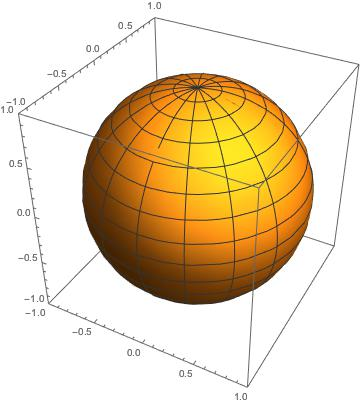
\includegraphics[width=5cm]{full.jpeg}
\caption{A full sphere}
\label{Fig1}}
\qquad
\begin{minipage}{5cm}
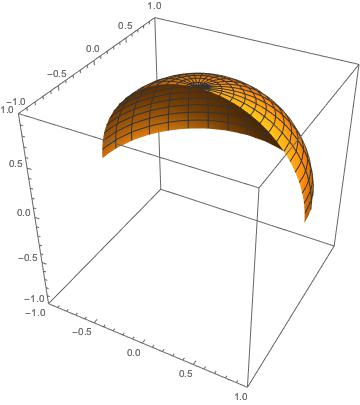
\includegraphics[width=5cm]{quarter.jpeg}
\caption{A subset of a sphere}
\label{Fig2}
\end{minipage}
\end{figure}

\end{example}


There are 2 main questions regarding parameterizations:
\begin{enumerate}
\item Once we're given a parametrization, how do we figure out what it looks like?
\item How do we find a parametrization for a given surface?
\end{enumerate}

Both can be hard to approach. 

\subsubsection*{The first question}
We have two main strategies:
\begin{enumerate}
\item Eliminate $u,v$ in the parametrization to find an expression that only involves $x, y, z$ and hope that it looks familiar.
\item Use grid curves.
\end{enumerate}

Let's explain both of them:

\begin{example} Suppose we are given the parametrization $$\vr(u,v)=\lg R\sin(u)\cos(v),R\sin(u)\sin(v),R\cos(u)\rg,\text{ for }(u,v)\in[0,\dfrac{\pi}{2}]\times[0,2\pi].$$ What does the surface look like?
\end{example}
\begin{solution} The identity $\sin^2(\theta)+\cos^2(\theta)=1$ is usually very useful in this type of problem. Squaring everything, we find $x^2=R^2\sin^2(u)\cos^2(v)$, $y^2=R^2\sin^2(u)\sin^2(v)$ and $z^2=R^2\cos^2(u)$, so $$x^2+y^2=R^2\sin^2(u),$$ and therefore $$x^2+y^2+z^2=R^2.$$ That tells us that our surface is \textbf{subset} of the sphere centered at the origin. Using the domain information, we may see that $u\in [0,\dfrac{\pi}{2}]\implies z\geq 0$, so our surface ends up being the upper semisphere of a sphere centered at the origin with radius $R$.
\begin{figure}[h]
\begin{center}
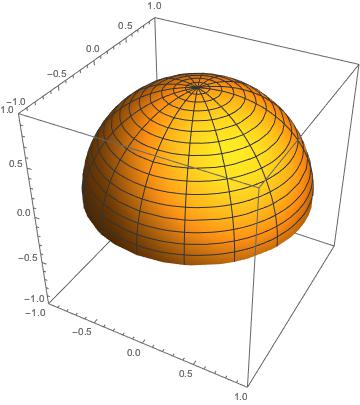
\includegraphics[scale=.3]{upperhalf.jpeg}
\end{center}
\end{figure}
\end{solution}

You can try to do the same thing with the following parametrization:
\begin{exercise}
$$\vr(u,v)=\lg (3+\cos(v))\cos(u),(3+\cos(v))\sin(u),\sin(v)\rg, \text{ for }(u,v)\in [0,2\pi]\times[0,2\pi]$$
\end{exercise}
Doing this exercise, you could find that $(\sqrt{x^2+y^2}-3)^2=1-z^2$. It doesn't look obvious what this looks like, so this brings us to the second strategy.


Note that if we set $v=v_0=const.$ and let $u$ run freely, $$r(u,v_0)$$ becomes a curve in $\R^3$, and curves are usually easier to visualize. Choosing several different values for $v_0$ and plotting the corresponding curves we can get a feeling of what the surface looks like. We can of course do the same by setting $u=u_0=const$. 

\begin{defn}
The curves $\vr(u_0,v)$ obtained by setting $u=u_0$ and $\vr(u,v_0)$ obtained by setting $v=v_0$ for various values of $u_0$ and $v_0$ are called \textbf{grid curves}.
\end{defn}

\begin{example}
As in the above exercise suppose $$\vr(u,v)=\lg (3+\cos(v))\cos(u),(3+\cos(v))\sin(u),\sin(v)\rg, \text{ for }(u,v)\in [0,2\pi]\times[0,2\pi].$$ By setting $v=v_0$ we find a circle that lies on the plane $z=\sin(v_0)$  with radius $(3+\cos(v_0))$, so as $v_0$ ranges from 0 to $2\pi$, the radius initially shrinks and starts growing again. At the same time, the plane on which the circle lies initially goes up, then down and up again. You can see those curves plotted in Figure \ref{fig3}.

Setting $u=u_0$, we find that $\dfrac{y}{x} =\tan(u_0),$ so the corresponding grid curve lives on the plane $y=\tan(u_0)x$ through the $z$ axis. Trying some easy values for $u_0$ like 0, $\pi/2,$ $\pi$, $3\pi/2$ we can see that the grid curves are circles. You can see them plotted in Figure \ref{fig4}.

The surface is plotted in figure \ref{fig5} (a torus).

\begin{figure}[h]
\minipage{0.32\textwidth}
  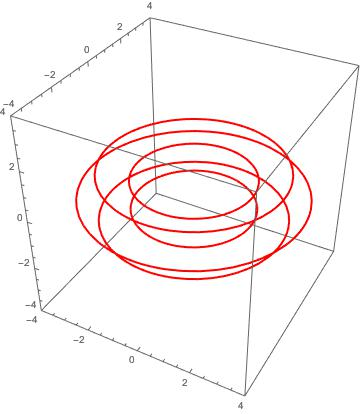
\includegraphics[width=\linewidth]{red.jpeg}
  \caption{Setting $v=v_0$.}\label{fig3}
\endminipage\hfill
\minipage{0.32\textwidth}
  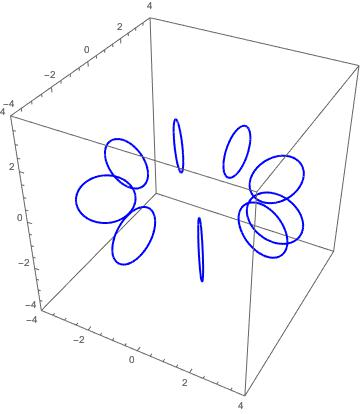
\includegraphics[width=\linewidth]{blue.jpeg}
  \caption{Setting $u=u_0$}\label{fig4}
\endminipage\hfill
\minipage{0.32\textwidth}%
  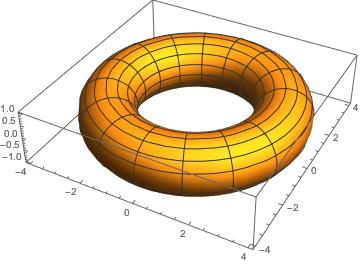
\includegraphics[width=\linewidth]{torus.jpeg}
  \caption{The full surface}\label{fig5}
\endminipage
\end{figure}
\end{example}


\begin{exercise}
In the parametrization given above for the sphere or radius $R$, check that the grid curves corresponding to $u=u_0$ are parallel circles and the curves corresponding to $v=v_0$ are meridians.
\end{exercise}

\subsubsection*{The second question}
It's hard to give a recipe on how to parametrize surfaces, but you can find some standard parametrizations in the handout, \href{http://sites.math.washington.edu/~neptamin/324Au17/Notes/Handout2/Handout2.pdf}{here}.

\subsection*{Tangent planes}
We've already seen a couple of methods to compute tangent planes to surfaces in different occasions:
\begin{enumerate}
\item Using impliticit differentiation
\item Using gradients.
\end{enumerate}
Now we'll see how to easily compute tangent planes to parametric surfaces. Suppose we have one, parametrized as $\vr(u,v)$, and suppose we want to find the tangent plane at $\vr(u_0,v_0)$. Recall from Math 126 that to write the equation of a plane it's enough to know a point through the plane and a normal vector, and $\vr(u_0,v_0)$, which is known, can serve as this point. So we only need to find a normal vector.

Let's remember the concept of grid curves we saw a bit earlier. The curve $\vr(u,v_0)$ passes through $\vr(u_0,v_0)$, so $$\vr_u(u_0,v_0):=\frac{\p}{\p u}\left (\vr(u,v_0)\right )_{|u=u_0}$$ is parallel to the tangent plane. Similarly, the curve $\vr(u_0,v)$ passes through $\vr(u_0,v_0)$, so $$\vr_v(u_0,v_0):=\frac{\p}{\p v}\left (\vr(u_0,v)\right )_{|v=v_0}$$ is parallel to the tangent plane too.

This means that their cross product $\rcross(u_0,v_0)$ is normal to the tangent plane at $\vr(u_0,v_0)$.

Finally \textbf{the equation of the tangent plane } to the parametric surface at $\vr(u_0,v_0)$ is given by $$\left( \lg x,y,z\rg-\vr(u_0,v_0)\right )\cdot\left (\rcross\right(u_0,v_0) )=0.$$

\begin{figure}[h]
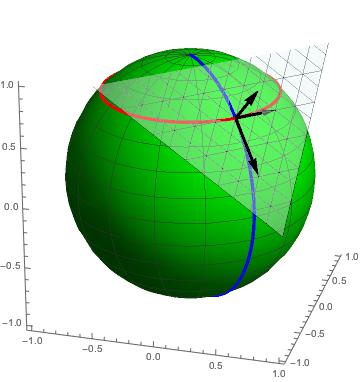
\includegraphics[scale=.3]{plane.jpeg}
\end{figure}

\begin{example}
Find the tangent plane to the unit sphere at $(\frac{1}{2},\frac{1}{2},\frac{\sqrt{2}}{2})$.
\end{example}
\begin{solution}
We use our favorite parametrization for the unit sphere:
$$\vr(u,v)=\lg \sin(u)\cos(v),\sin(u)\sin(v),\cos(u)\rg,\text{ for }(u,v)\in[0,\pi]\times[0,2\pi].$$
Note that $\vr(\frac{\pi}{4},\frac{\pi}{4})=(\frac{1}{2},\frac{1}{2},\frac{\sqrt{2}}{2})$.
Then, we have $$\vr_u(u,v)=\lg \cos(u)\cos(v),\cos(u)\sin(v),-\sin(u)\rg$$ and $$\vr_v(u,v)=\lg -\sin(u)\sin(v),\sin(u)\cos(v),0\rg.$$
Therefore, for $u=\frac{\pi}{4}$ and $v=\frac{\pi}{4}$ we have 
$$\vr_u(\frac{\pi}{4},\frac{\pi}{4})=\lg \frac{1}{2},\frac{1}{2},-\frac{\sqrt{2}}{2}\rg$$
$$\vr_v(\frac{\pi}{4},\frac{\pi}{4})=\lg -\frac{1}{2},\frac{1}{2},0\rg$$

So $$\rcross(\frac{\pi}{4},\frac{\pi}{4})=\lg \frac{\sqrt{2}}{4},\frac{\sqrt{2}}{4},\frac{1}{2}\rg$$ and therefore the tangent plane is given by $$(x-\frac{1}{2})\frac{\sqrt{2}}{4}+(y-\frac{1}{2})\frac{\sqrt{2}}{4}+(z-\frac{\sqrt{2}}{2})\frac{1}{2}=0.$$
\end{solution}

\subsection*{Surface Area}
We will give a formula that allows us to compute the surface area of a parametric surface.

The \textbf{area of a surface} $S$ parametrized by $\vr(u,v)$, $(u,v)\in D$, is given by \begin{equation}\label{eq1}A(S)=\iint_D|\rcross(u,v)|dA.
\end{equation} We will denote $dS:=|\rcross|dA$ so that we may write $$A(S)=\iint_D dS.$$

In the special case that $S$ is the graph of a function $f(x,y)$, $(x,y)\in D$, we may parametrize $S$ by $$\vr(u,v)=\lg u,v,f(u,v)\rg,\text{ for }(u,v)\in D.$$ With this parametrization, \eqref{eq1} becomes \begin{equation}\label{eq2}A(S)=\iint_D\sqrt{1+\left (\frac{\p f}{\p x}\right )^2+\left( \frac{\p f}{\p y}\right )^2}dA.\end{equation}

Equation \eqref{eq2} can be very useful because surfaces are very frequently expressed as graphs of functions.

\begin{example}
Find the surface area of the sphere of radius $R$.
\end{example}

\begin{solution}
${}$
\newline
\textbf{1st way: Using \eqref{eq1}.}
We can assume that the sphere is centered at the origin. The equation of the sphere is then $$x^2+y^2+z^2=R^2$$ and we can parametrize it as $$\vr(u,v)=\lg R\sin(u)\cos(v),R\sin(u)\sin(v),R\cos(u)\rg,\text{ for }(u,v)\in[0,\pi]\times[0,2\pi].$$


Then we have $$\vr_u(u,v)=\lg R\cos(u)\cos(v),R\cos(u)\sin(v),-R\sin(u)\rg$$ and $$\vr_v(u,v)=\lg -R\sin(u)\sin(v),R\sin(u)\cos(v),0\rg,$$
so $$\rcross(u,v)=\lg R^2\sin^2(u)\cos(v),R^2\sin^2(u)\sin(v),R^2\cos^2(v)\cos(u)\sin(u)+R^2\sin^2(v)\cos(u)\sin(u)\rg$$

which implies
$$|\rcross(u,v)|=R^2\sin(u).$$ Therefore, $$A(S)=\int_0^{2\pi}\int_0^\pi R^2\sin(u)dudv=4\pi R^2.$$

\noindent\textbf{2nd way: Using \eqref{eq2}.}
The sphere is \textbf{not} the graph of a function (why?), but both its upper and lower hemisphere \textbf{are} graphs of functions and they have the same surface area. So we'll consider the function \begin{equation}\label{upper}z=f(x,y)=\sqrt{R^2-x^2-y^2}\end{equation}  representing the upper hemisphere. To find the domain of integration, we intersect with the $xy$ plane and find, by \eqref{upper}, $$z=0\implies x^2+y^2=R^2.$$ So, the domain of integration has to be the disk $$D=\{(x,y):x^2+y^2\leq R^2\}.$$

Then we compute partial derivatives and find $$f_x(x,y)=\frac{-2x}{2\sqrt{R^2-x^2-y^2}}$$ and $$f_y(x,y)=\frac{-2y}{2\sqrt{R^2-x^2-y^2}}.$$ Therefore, the area $H$ of the upper hemisphere is\begin{align*}
H=&\iint_D\sqrt{(f_x(x,y))^2+(f_y(x,y))^2+1}dA\\
=&\iint_D\frac{R}{\sqrt{R^2-x^2-y^2}}dA\\
=&\int_0^{2\pi}\int_0^R\frac{Rr}{\sqrt{R^2-r^2}}drd\theta\\
=&\int_0^{2\pi}\int_{R}^0-\frac{R}{2}u^{-\frac{1}{2}}dud\theta\\
=&2\pi R^2.
\end{align*}

To find the total surface area of the sphere we multiply $\times 2 $ and we find $$A(S)=4\pi R^2.$$
\end{solution}

\end{document}

